%% LyX 2.3.6.1 created this file.  For more info, see http://www.lyx.org/.
%% Do not edit unless you really know what you are doing.
\documentclass[english]{article}
\usepackage[T1]{fontenc}
\usepackage[latin9]{inputenc}
\usepackage{amsbsy}
\usepackage{amstext}
\usepackage{amssymb}
\usepackage{graphicx}
\usepackage{babel}
\begin{document}

\section{SIR}

Let's consider $n$ classes (example: age) of individuals and let
$s_{k}$,$i_{k}$,$r_{k}$ be the fraction of susceptibles, infectious
and recovered individuals in the $k^{th}$ class. The SIR equations
for such an heterogeneous population are:
\begin{equation}
\begin{array}{c}
\partial_{t}s_{k}=-s_{k}\sum_{l}\beta_{kl}i_{l}\\
\partial_{t}i_{k}=i_{k}\sum_{l}\beta_{kl}s_{l}-\gamma_{k}i_{k}\\
\partial_{t}r_{k}=\gamma_{k}i_{k}
\end{array}\label{eq:sir}
\end{equation}
with the conservation law $1=s_{k}+i_{k}+r_{k}$ (i.e., we are confined
in the simplex $\boldsymbol{s}\geq0$,$\boldsymbol{r}\geq0$,$\boldsymbol{s}+\boldsymbol{r}\leq\boldsymbol{1}$).
Conservation comes from the fact that $\partial_{t}\sum_{k}\left(s_{k}+i_{k}+r_{k}\right)=0$.
Using $i_{k}=\gamma_{k}^{-1}\partial_{t}r_{k}$, the evolution of
the epidemics plane follows the law 
\begin{equation}
\partial_{t}\ln s_{k}=-\sum_{l}\beta_{kl}\gamma_{l}^{-1}\partial_{t}r_{l}\label{eq:main}
\end{equation}
i.e. (in vector form) $\partial_{t}\ln s=-\mathcal{R}\partial_{t}r$
where the matrix $\mathcal{R}=\textrm{diag}(\gamma)^{-1}\beta$ is
the basic reproduction number matrix. Thus, defining $y=\ln s$, SIR
epidemics have the form 
\begin{equation}
y^{SIR}=\ln s_{0}-\mathcal{R}\left(r-r_{0}\right)\label{eq:straight}
\end{equation}
. 

An epidemic ends when $\boldsymbol{i}=0$, i.e. on the hyper-surface
$\boldsymbol{s}+\boldsymbol{r}=\boldsymbol{1}$; in fact on these
point $\partial_{t}\boldsymbol{s}=\partial_{t}\boldsymbol{r}=\boldsymbol{0}$
(eq.\ref{eq:sir}). In the $r-y$ plane, these points define the boundary
$\Omega$ (also called the disease-free set) defined by the concave,
monotonously decreasing function (also called the disease-free equilibrium
curve)
\begin{equation}
y^{\Omega}=\ln\left(1-r\right)\label{eq:boundary}
\end{equation}
; thus, the end of an epidemic corresponds to the rightmost intersection
$P^{\infty}$ of eq.\ref{eq:straight} with eq. \ref{eq:boundary}.
In general, $P^{\infty}$ will depend from the initial values of $r_{0}$,$s_{0}$.

To define stability, let's consider the total fraction of infected
$i=\sum_{k}i_{k}$; a boundary point $P$ is stable if 
\begin{equation}
\partial_{t}i=\sum_{k}\gamma_{k}i_{k}\left(\sum_{l}\mathcal{R}_{kl}s_{l}-1\right)<0\label{eq:i_decreases}
\end{equation}
i.e. $\mathcal{R}\boldsymbol{s}<\boldsymbol{1}$. Notice that, since
$\Omega$ is strictly concave, $\left.\partial_{t}i\right|_{P^{\infty}}=0$
as expected. A particular case is the ``initial'' epidemics, i.e.
the one starting from $r_{0}=0$, $i_{0}\to0$ (i.e. $s_{0}\to1$,
$y_{0}\to0$). In this point $s_{l}\sim1$ and $\partial_{t}i\sim\sum_{k}\gamma_{k}i_{k}\left(\sum_{l}\mathcal{R}_{kl}-1\right)$
that is stable ($<0$) if $\sum_{l}\mathcal{R}_{kl}<1$; this is a
generalization of the $1d$ case where the critical value for an epidemic
to start is $R>1$. 

Let's consider a boundary point $P^{\Omega}=(\boldsymbol{s}^{\Omega},\boldsymbol{r}^{\Omega})$
with $R\boldsymbol{s}^{\Omega}<\boldsymbol{1}$; this point is stable
against any perturbation $0<i_{l}<$ $1-\sum_{l}\mathcal{R}_{kl}s_{l}^{\Omega}$
(see eq. \ref{eq:i_decreases}), since in this boundary (that is non
empty if $\mathcal{R}$ is an invertible matrix) is non empty (essentially,
I need that $\sum_{l}\mathcal{R}_{kl}s_{l}^{\Omega}>0$ strictly).

Thus, I can define the frontier $\omega\subset\Omega$
\[
\omega=\left\{ P\in\Omega:R\boldsymbol{s}^{\Omega}=\boldsymbol{1}\right\} 
\]
separating the unstable set $\Omega^{u}$ where $R\boldsymbol{s}>\boldsymbol{1}$
from the stable set $\Omega^{s}$. The set $\omega$ is the $d$-dimensional
equivalent of the herd immunity threshold.

\section{Vaccines}

In SIR, recovered individuals are considered immune. Thus, a vaccination
policy consists in moving a population from a point $(\boldsymbol{s}_{0},\boldsymbol{r}_{0})$
(tipically/hopefully $s_{k}=1$, $r_{k}=0$) to a point $(\boldsymbol{s}_{\Omega},\boldsymbol{r}_{\Omega})\in\Omega^{s}$.
A minimal vaccination policy is a point belonging to $\omega$. Since
an epidemic can have different impacts on the various classes (i.e.
mortality rates per age classes), one can consider the advantage of
having a fraction $r_{k}$ of recovered individuals in the $k^{th}$
class generated through the vaccine and not through having been infected.
Let's assume that we start vaccination from a point $P_{0}=(\boldsymbol{s}_{0},\boldsymbol{r}_{0})$.
This means that we have $\boldsymbol{i}_{0}=\boldsymbol{1}-\boldsymbol{r}_{0}-\boldsymbol{s}_{0}$
infectious individuals; let's suppose we can vaccine only sane individuals,
i.e. a fraction $\boldsymbol{r}_{V}<\boldsymbol{s}_{0}$. if we ``land''
on a stable point of $\Omega$, we will end up with $\boldsymbol{r}_{SIR}=1-\boldsymbol{s}_{0}$
recovered individuals (the $\boldsymbol{r}_{0}$ initial ones plus
the $\boldsymbol{i}_{0}$ that were infected ) and $\boldsymbol{r}_{V}$
vaccined individuals, i.e. $\boldsymbol{r}_{\Omega}=\boldsymbol{r}_{V}+\boldsymbol{r}_{SIR}$. 

Let's try a simple example: let $\mu_{k}$ be the mortality rate in
the $k^{th}$ class and suppose that vaccination has an irrelevant
cost. Thus, a best policy $\boldsymbol{r}_{V}$ would be one that
optimezes the problem
\[
\begin{array}{c}
\min\boldsymbol{\mu}\cdot\boldsymbol{r}\\
\textrm{s.t. }\boldsymbol{r}+\boldsymbol{1}-\boldsymbol{s}_{0}\in\omega
\end{array}
\]
that, since $\omega$ is convex and bounded (it is the intersection
of a linear constrain with a strictly convex surface), has a unique
solution (check, this is an ansatz !!!).

Another simple example: let's consider a vaccination policy with cost
$c_{V}\left(\boldsymbol{r}\right)$. The best policy would be the
$\boldsymbol{r}_{V}$ that minimizes the problem:
\[
\begin{array}{c}
\min c_{V}\left(\boldsymbol{r}\right)\\
\textrm{s.t. }\boldsymbol{r}+\boldsymbol{1}-\boldsymbol{s}_{0}\in\omega
\end{array}
\]
that is a generalization of the previous and, if $\omega$ is convex
and bounded, would have a unique solution again if $c$ is monotonic.

A more complex optimization problem would be the case where I have
a limited amount $M$ of vaccine, so that I can vaccine part of the
population and let the other part get the infection. Let $d(\boldsymbol{r})$
the damage to the national health system given by a fraction $\boldsymbol{r}$
of the population being infected. Under such circumstances, the optimal
$\boldsymbol{r}_{V}$ solves the problem
\[
\min c_{V}\left(\boldsymbol{r}\right)+d\left(\boldsymbol{r}_{\infty}\left(\boldsymbol{r}+\boldsymbol{r}_{0}\right)\right)
\]
where $\boldsymbol{r}_{\infty}\left(\boldsymbol{r}+\boldsymbol{r}_{0}\right)$
is the intersection of eq.\ref{eq:straight} with initial conditions
$\left(\boldsymbol{r}_{0}+\boldsymbol{r},\boldsymbol{s}_{0}\right)$
to the boundary. Here I have relaxed the condition $\boldsymbol{r}\in\omega$
since $\boldsymbol{r}_{\infty}$ cannot be not obliged to belong to
$\omega$ but surely belongs by construction to $\Omega^{s}$.

\section{Majorants and minorants in n dimensions}

The point $\mathcal{R}\boldsymbol{s}^{*}=\boldsymbol{1}$is the separating
point between stable and unstable points. 

To the matrix $\mathcal{R}$ we can associate the $n^{2}$ points
\[
\boldsymbol{s}_{ij}^{max}=\mathcal{R}_{ij}^{-1}\boldsymbol{1}_{j}
\]
; thus, $\boldsymbol{s}_{ij}^{max}=\left(0,\ldots,0,\mathcal{R}_{ij}^{-1},0,\ldots,0\right)$
has all $0$ components but the $j^{th}$ that is (with an abuse of
notation) $s_{ij}^{max}=\mathcal{R}_{ij}^{-1}$\footnote{Notice that for a matrix $\mathcal{A}$, $\mathcal{A}\boldsymbol{1}_{j}=\mathcal{A}_{j}$
where $\mathcal{A}_{j}$ is the $j^{th}$ column of $\mathcal{A}$
and that $\boldsymbol{1}_{i}^{T}\mathcal{A}\boldsymbol{1}_{j}=\mathcal{A}_{ij}$.
Thus, If we define $\mathcal{S}:\mathcal{S}_{ij}=\mathcal{R}_{ij}^{-1}$,
$\mathcal{S}_{ij}=\boldsymbol{1}_{i}^{T}\mathcal{S}\boldsymbol{1}_{j}$.}. By construction, $\mathcal{R}\boldsymbol{s}_{ij}^{max}=\boldsymbol{1}_{j}$.
Moreover, the n vectors $\left\{ \boldsymbol{s}_{i1}^{max},\ldots,\boldsymbol{s}_{in}^{max}\right\} $
constitute an orthogonal basis in $\mathbb{R}^{n}$.

Let's consider the point $\boldsymbol{s}^{max}=\sum_{i}\boldsymbol{s}_{ii}^{max}$;
if $\mathcal{R}_{ii}>1$, this is interior to the domain $\mathbf{0}\leq\mathbf{s}\leq\mathbf{1}$.
Thus, there are points $\mathbf{s}>\mathbf{s}^{max}$; for such points,
$\mathcal{R}\mathbf{s}>\mathcal{R}\mathbf{s}^{max}\geq\mathcal{D}\mathbf{s}^{max}=\mathbf{1}$where
$\mathcal{D}_{ij}=\delta_{ij}\mathcal{R}_{ij}$, i.e. $\mathcal{D}$
is the diagonal matrix associated to $\mathcal{R}$. Thus, $\boldsymbol{s}^{*}$
belongs to the hypercube $0\leq\boldsymbol{s}\leq\boldsymbol{s}^{max}$.

Let's consider the convex set $\boldsymbol{s}=\sum_{i}\alpha_{i}\boldsymbol{s}_{ii}^{max}=diag\left(\boldsymbol{\alpha}\right)\mathbf{s}^{max}$
with $\sum_{i}\alpha_{i}=1$; such a set belongs to the hyperplane
$\boldsymbol{s}\cdot\boldsymbol{s}^{max}=1$. Since $\alpha_{i}\leq1$,
for such points $\mathcal{R}\boldsymbol{s}=\sum_{i}\alpha_{i}\mathcal{R}\boldsymbol{s}_{ii}^{max}=\sum_{i}\alpha_{i}\boldsymbol{1}_{j}<\boldsymbol{1}$.
Thus, $\boldsymbol{s}^{*}$ belongs to the exterior of the plane $\boldsymbol{s}:\boldsymbol{s}\cdot\boldsymbol{s}^{max}>1$.
In fig.\ref{fig:Majorants-and-minorants} we show an example in $n=2$
dimensions.
\begin{figure}
\begin{centering}
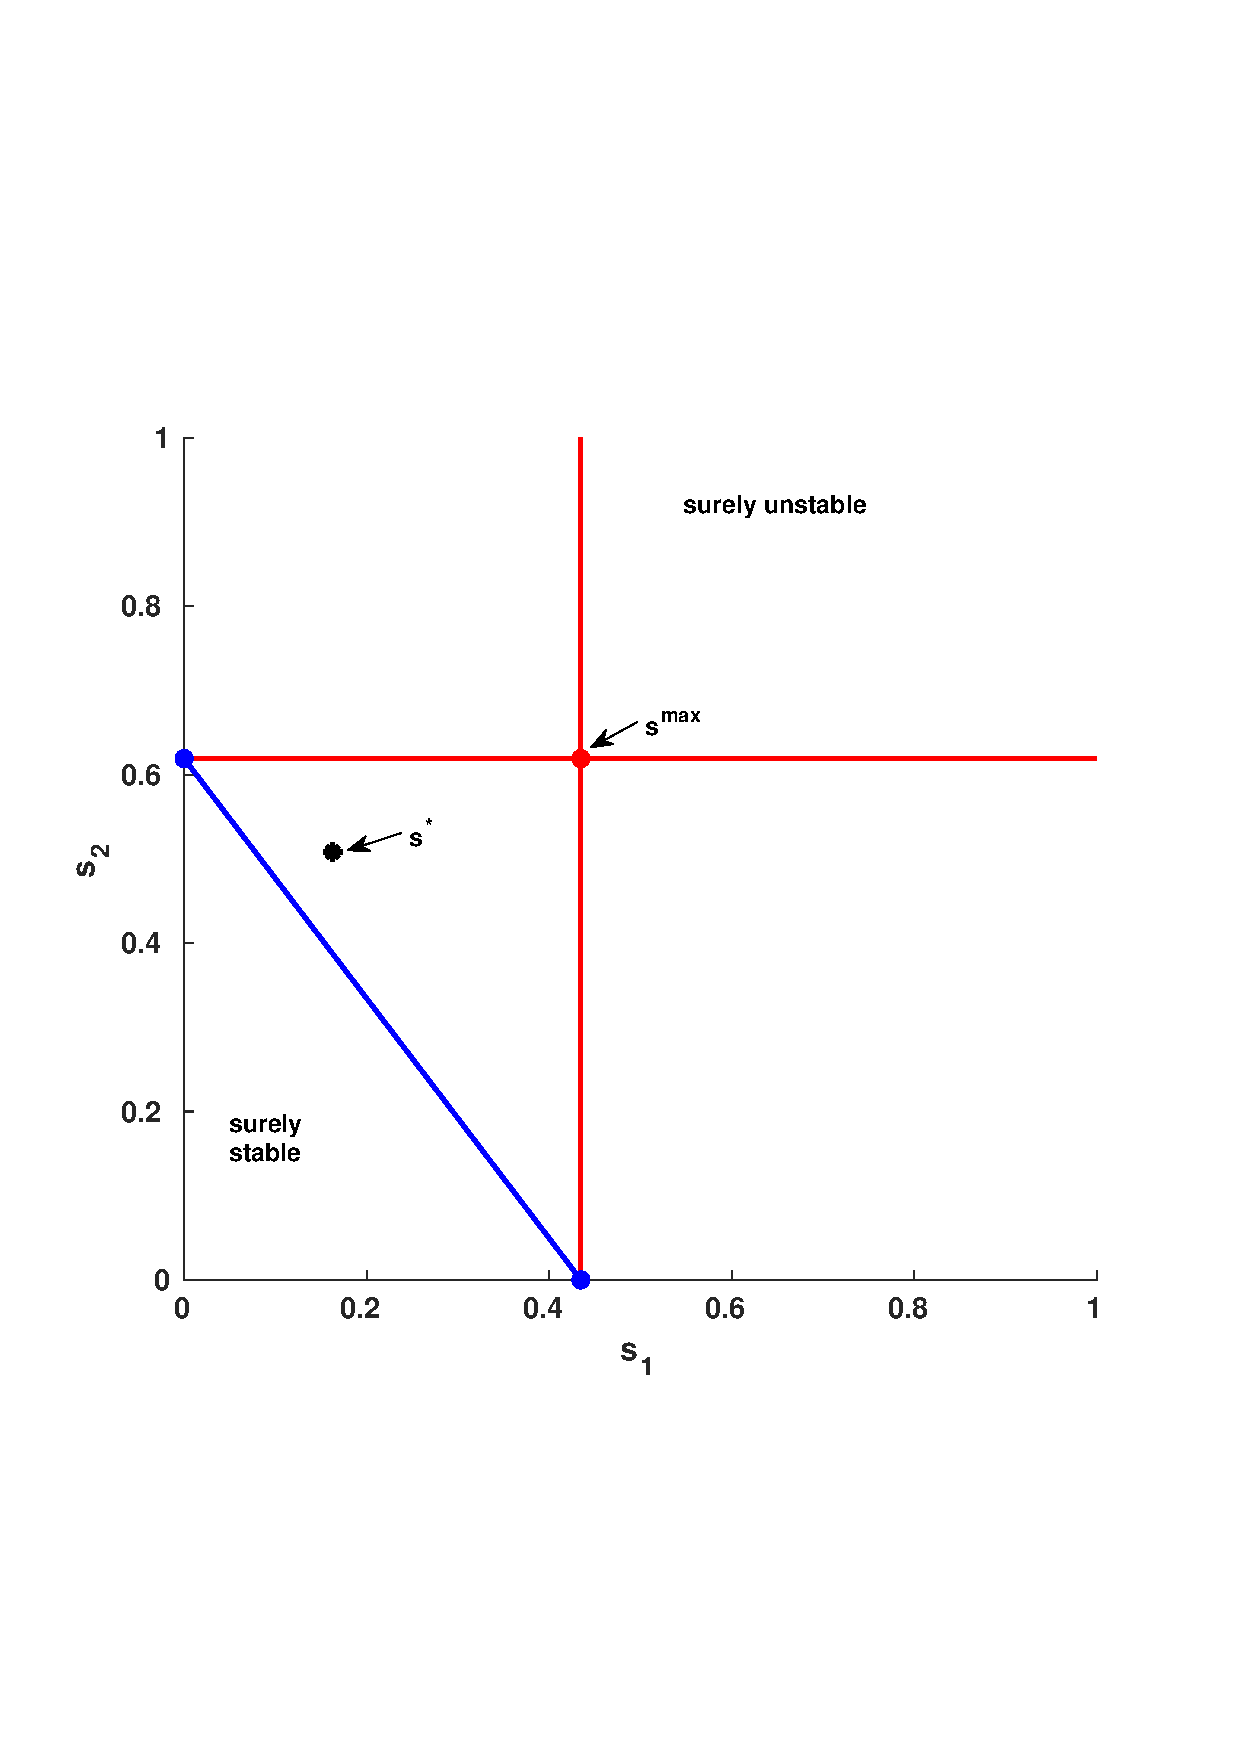
\includegraphics[width=0.7\columnwidth]{majmin2d}
\par\end{centering}
\caption{Majorants and minorants\label{fig:Majorants-and-minorants}}
\end{figure}


\section{Solution in n dimensions}

Let's consider the convex set $\boldsymbol{s}=\sum_{i}\alpha_{i}\boldsymbol{s}_{ij}^{max}$
with $\sum_{i}\alpha_{i}=1$; such a set belongs to the hyperplane
$\boldsymbol{s}\cdot\boldsymbol{\theta}^{j}=1$ where we have defined
$\boldsymbol{\theta}^{j}=\sum_{i}\boldsymbol{s}_{ij}^{max}$. Since
$\alpha_{i}\leq1$, for such points $\left(\mathcal{R}\boldsymbol{s}\right)_{j}=\left(\sum_{i}\alpha_{i}\mathcal{R}\boldsymbol{s}_{ij}^{max}\right)_{j}=\left(\sum_{i}\alpha_{i}\boldsymbol{1}_{j}\right)_{j}=1$\footnote{More esplicit calculation: $\left(\mathcal{R}\boldsymbol{s}\right)_{j}=\sum_{i}\alpha_{i}\sum_{k}\mathcal{R}_{ik}\left(\boldsymbol{s}_{ij}^{max}\right)_{k}=\sum_{i}\alpha_{k}=1$,
since $\sum_{k}\mathcal{R}_{ik}\left(\boldsymbol{s}_{ij}^{max}\right)_{k}=\sum_{k}\mathcal{R}_{ik}\mathcal{R}_{ij}^{-1}\delta_{jk}$.}; thus, this plane separate the points where the $j^{th}$ component
of the SIR model is unstable (i.e. when $\boldsymbol{s}\cdot\boldsymbol{\mu}^{j}>1$,
$\partial_{t}i_{j}>0$ and $i_{j}$ reaches a maximum on $\boldsymbol{s}\cdot\boldsymbol{\mu}^{j}=1$).
Thus, $\boldsymbol{s}^{*}$ belongs to the set $\Theta^{j}=\left\{ \boldsymbol{s}:\boldsymbol{s}\cdot\boldsymbol{\theta}^{j}\leq1\right\} $.
Moreover, at the intersection $\bigcap_{j}\Theta^{j}$ I have that
$\forall j\left(\mathcal{R}\boldsymbol{s}\right)_{j}=1$ i.e. $\mathcal{R}\boldsymbol{s}=\boldsymbol{1}$
i.e. $\boldsymbol{s}^{*}\in\bigcap_{j}\Theta^{j}$; if $\mathcal{R}$
is invertible, $\bigcap_{j}\Theta^{j}=\left\{ \boldsymbol{s}^{*}\right\} $.
See fig.\ref{fig:Stability-boundaries} for an example in $n=2$ dimensions.
Notice that in $n=2$ dimensions I have $2^{n}=4$ convex sets:
\begin{enumerate}
\item $\boldsymbol{s}\cdot\boldsymbol{\theta}^{1}<1,\boldsymbol{s}\cdot\boldsymbol{\theta}^{2}<1$
corresponding to the stable set $\partial_{t}i_{1}<0,\partial_{t}i_{2}<0$
\item $\boldsymbol{s}\cdot\boldsymbol{\theta}^{1}>1,\boldsymbol{s}\cdot\boldsymbol{\theta}^{2}<1$
corresponding to the $s_{1}$-unstable/$s_{2}$-stable set $\partial_{t}i_{1}>0,\partial_{t}i_{2}<0$
\item $\boldsymbol{s}\cdot\boldsymbol{\theta}^{1}<1,\boldsymbol{s}\cdot\boldsymbol{\theta}^{2}>1$
corresponding to the $s_{2}$-unstable/$s_{1}$-stable set $\partial_{t}i_{1}<0,\partial_{t}i_{2}>0$
\item $\boldsymbol{s}\cdot\boldsymbol{\theta}^{1}>1,\boldsymbol{s}\cdot\boldsymbol{\theta}^{2}>1$
corresponding to the unstable set $\partial_{t}i_{1}>0,\partial_{t}i_{2}>0$
\end{enumerate}
In general, there will be $2^{n}$ sets corresponding to the possible
stable/unstable combinations. \footnote{Probably useless: let $\chi\in\left\{ 0,1\right\} ^{n}$and associate
to it the set $\Phi^{\chi}$ such that $\partial_{t}i_{k}<0$ if $\chi_{k}=1$,
$\partial_{t}i_{k}>0$ otherwise, i.e. 

\[
\Phi^{\chi}=\bigcap_{k:\chi_{k}=1}\Theta^{k}
\]
; thus, we have that to $\Phi^{\boldsymbol{1}}$ is the stable set,
that for $\boldsymbol{0}<\chi<\boldsymbol{1}$ $\Phi^{\chi}$ is a
set with at least $\sum_{k}\chi_{k}$ stable directions and by convention
we associate to $\chi=\boldsymbol{0}$ the set 
\[
\Phi^{\boldsymbol{0}}=\Psi-\bigcup_{\chi<\boldsymbol{1}}\Phi^{\chi}
\]
where we indicate with $\Psi$ the whole orthant $\boldsymbol{0}<\boldsymbol{s}<\boldsymbol{1}$.
For such sets, we have that $\chi_{A}<\chi_{B}\to\Phi^{\chi_{A}}\subset\Phi^{\chi_{B}}$;
also, the number of ``unstable'' directions is an instability index
$u_{\chi}=\sum_{k}\chi_{k}$. }

\begin{figure}
\begin{centering}
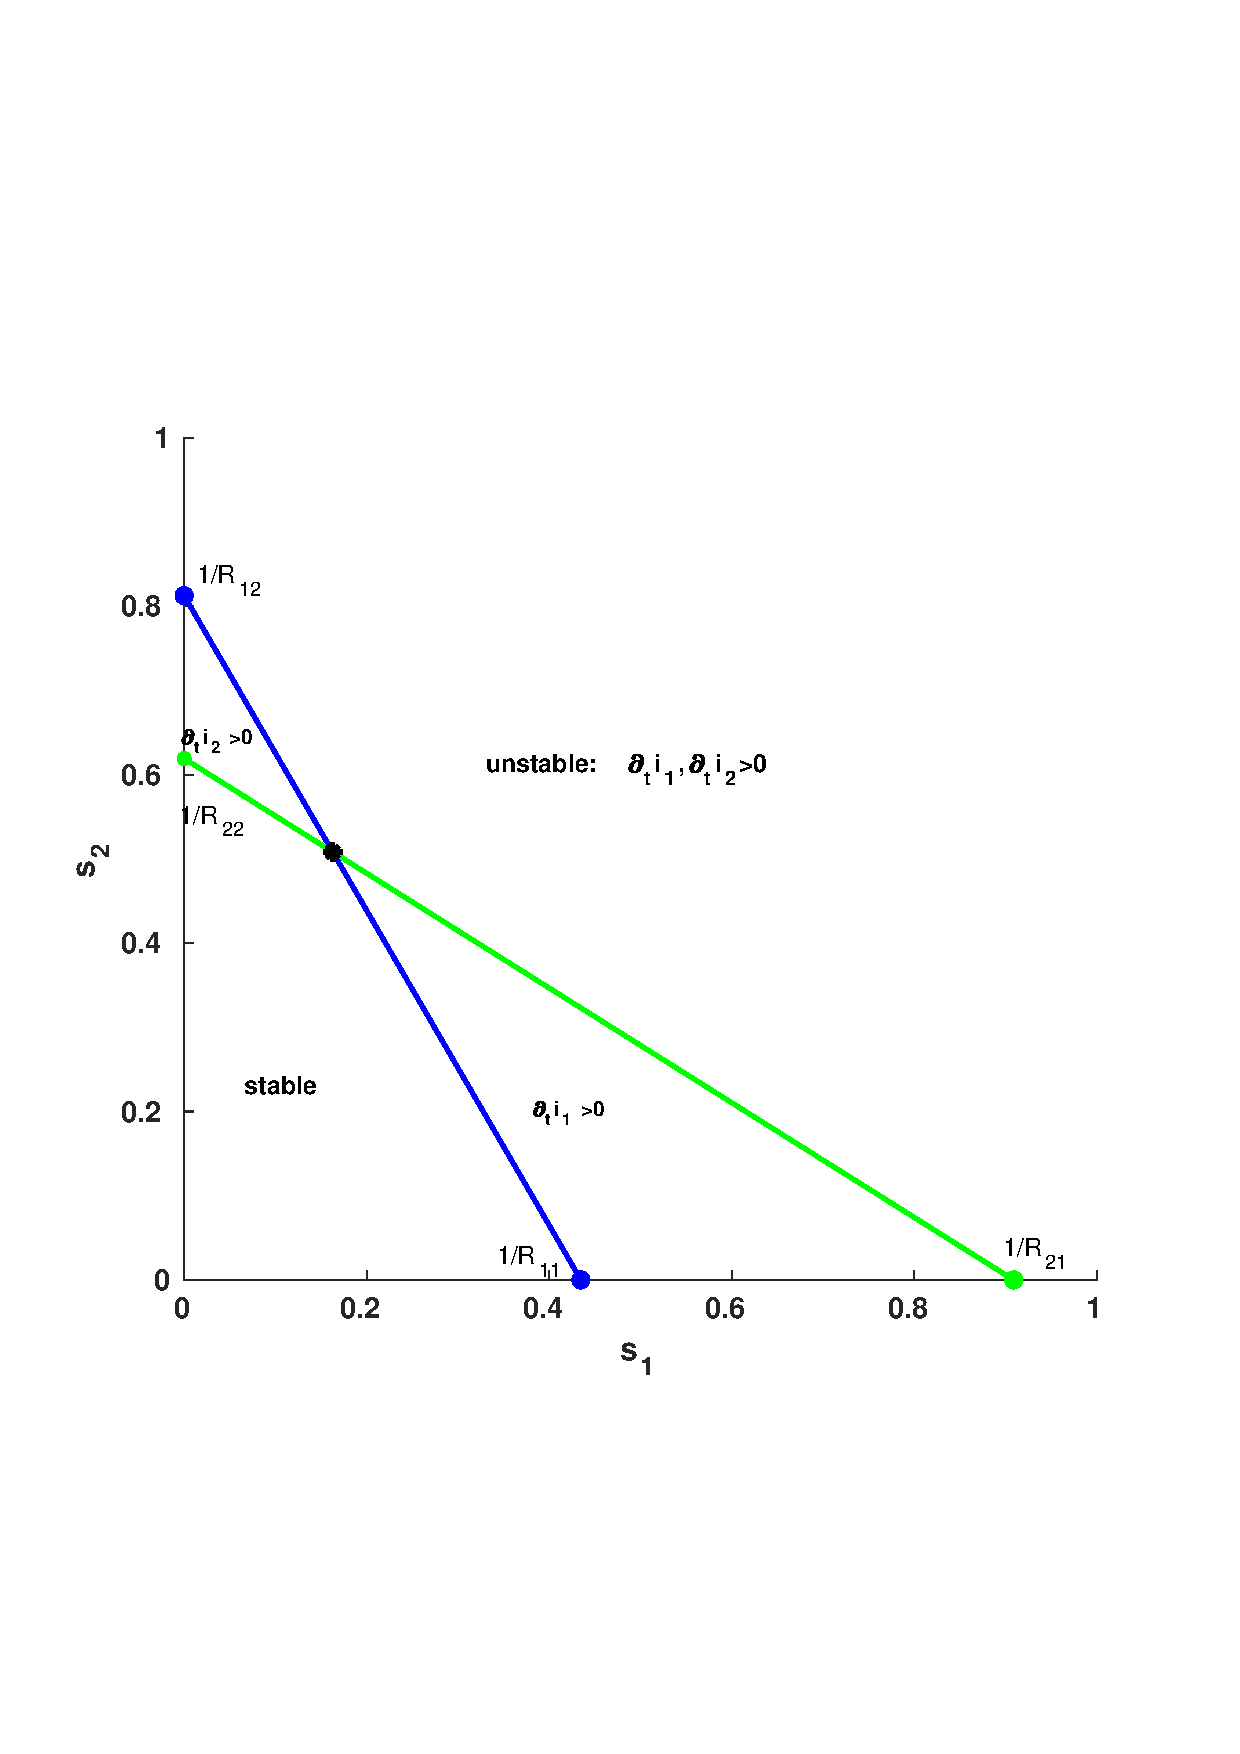
\includegraphics[width=0.7\columnwidth]{crit2d}
\par\end{centering}
\caption{Stability boundaries\label{fig:Stability-boundaries}}
\end{figure}

\end{document}
